% referee comments (minor)
%3. Section 4.3: I suggest putting the numeric results for the chi-squared agreement score (paragraph 2) and silhouette score (paragraph 4) into tables to improve their readability.

%4. Section 4.2.1 - typo - space needed between the symbol for "angstroms" and the word following it (e.g., "range", "break" - in the new bolded text).

\section{RESULTS AND DISCUSSION}
\label{sec: result}

    In this section we show the results of the neural networks and K-means clustering trained using the \citetalias{Kinney96} template spectra.
    Training with \citetalias{Kinney96} templates results in networks or clusters that have regions corresponding to galaxies of known morphological type. 
    The trained networks or clusters can then be used to categorize other galaxies.

    The first step in categorizing galaxies is choosing the number of classes.
    In the K-means method empty clusters are not allowed; 
    hence a $K=12$ clustering would produce one-object clusters as in Fig.~\ref{fig: k96}.
    We did not want to have too dense or too sparse clusters.
    Therefore we chose the number of clusters in the K-means clustering method to be $K=4$.
    Since empty neurons are allowed in SOMs, finding an optimal number of neurons for SOM networks is more subtle than just specifying a number of clusters. 
    In order to find a sufficient size for the trained neural networks, we created maps with sizes ranging from $1\times2$ to $50\times50$.
    Varying the grid size of the maps helps us to monitor whether tighter grouping of galaxies is due to their similar properties or a lack of map space to separate them.
    Based on the size of the data and SOM results, we found the optimum grid size to be $1\times22$ and $12\times12$ in 1D and 2D maps, respectively. 
    For each grid we created different SOMs with different learning factors, neighbourhood distances, and number of iterations to find the optimum.
   
    We started our analysis by creating 1D SOMs and K-means clustering. 
    First, we created SOMs with only two neurons ($1\times2$ map), and then increased the number of neurons one at a time (Section~\ref{sec: 1Dt}).
    We performed K-means clustering on the \citetalias{Kinney96} templates (Section~\ref{sec: Kmeansvssom}) and compared 
   the results with the results of the $1\times4$-sized 1D SOMs (Section~\ref{sec: Kmeansvssom}).
    For 2D networks (Section~\ref{sec: 2D}), we found the optimum size for the network to be $12\times12$ and created two types of SOM to show different applications of 2D SOMs.
    In Section~\ref{sec: Kmeansvssomvsann} we compare the results of the different classification in several ways. 
    For each generated neural network, we compare the results with the \citetalias{Kinney96} categorization.
    We also use these networks to classify the \citetalias{Hossein12} galaxy sample, and compare this classification with that from the supervised networks in \citetalias{Hossein12} and with K-means clustering.



    \subsection{One-dimensional self-organizing maps}
    \label{sec: 1D_somz}
        \subsubsection{Training the networks}
        \label{sec: 1Dt}
            To start our classification, we assumed that galaxies can be divided into only two general types, quiescent and starburst.
            This corresponds to a network with only two neurons.
            We increased the size of the map gradually until the 12 input samples divide into the 12 neurons. 
        
            Figs.~\ref{fig: 1by2T} --~\ref{fig: 1by22T} show the results of the training networks.  
            The upper part of the figures shows the neurons and the relative distances between their weights. 
            As mentioned in Section~\ref{sec: method_somz}, an increase in the darkness of colours between neurons represents an increase in relative distance between the neurons.
            The lower panels of the figures show the number of \citetalias{Kinney96} templates that are placed in each neuron. 
            \begin{figure}
                \begin{subfigure}[b]{0.45\textwidth}
                    \centering
                  \includegraphics[width=\textwidth]{images0.01/1d/dist_1_by_2.png}
                \end{subfigure}
                \hfill
                \begin{subfigure}[b]{0.45\textwidth}
                    \centering \includegraphics[width=\textwidth]{images0.01/1d/hit_t_1_by_2.png}
                \end{subfigure}
                \caption[Results of training network in $1\times2$~grid]{Results of training network in $1\times2$~grid. The upper panel is a distance map and the lower panel is a hit map. In this network, 5 of the templates from \citet{Kinney96} are categorized as quiescent galaxies and the rest are starbursts. Because of their strong emission lines, Sc galaxies are moved towards the starburst ones.}
                 \label{fig: 1by2T}
            \end{figure}
        
        
            In the upper map in Fig.~\ref{fig: 1by2T}, the dark colour between two neurons indicates that the relative distance between these two groups is high, and these two groups are distinguishable.
            In the lower part of Fig.~\ref{fig: 1by2T}, we see that the templates are divided into two groups of 5 and 7.
            Although we know from \citetalias{Kinney96} and \citetalias{Hossein12} that 6 of the templates are quiescent and the other 6 are starbursts, the SOM results show 5 of the galaxies in one group and the other 7 in the second group.
            In this method, the Sc template has been categorized as starburst due to the relatively higher disk stellar population relative to that of the bulge. 
            According to \citetalias{Kinney96}, Sc galaxies are considered to be late Hubble type galaxies which have  flatter spectra compared to other quiescent galaxies. 
            

            Fig.~\ref{fig: 1by3T} shows the results of the training in a 1$\times$3 network.
            In these plots we force the galaxies to be categorized in a maximum of three groups. 
            If the templates in Fig.~\ref{fig: 1by2T} truly belonged in two groups, they would be grouped into two groups in this network, even when we try to cluster them into three. 
            However, in the lower panel of Fig.~\ref{fig: 1by3T}, we can see that the middle node contains two templates.
            These two templates, which are separated from the group of starburst templates in the lower part of Fig.~\ref{fig: 1by2T},  are the SB5 and SB6 types.
            In the upper plot of Fig.~\ref{fig: 1by3T}, the colour between two right neurons is black and the colour between two left neurons is white. 
            The black colour indicates that the left neuron has the most differences with the other two groups,
            while the white colour shows that the two right neurons are very similar to one another. 
            
            Comparing Fig.~\ref{fig: 1by2T} to Fig.~\ref{fig: 1by3T} shows that the starburst templates are divided into two groups. 
            Based on the colours between these two groups, we conclude that they are more similar to each other than to the ones in the left neurons; both groups are starbursting and have strong emission lines.
            On the other hand, the SB5 and SB6 templates have the highest internal extinctions; this causes the spectra to become flatter at shorter wavelengths. 
            The flatter UV spectra make these two templates more similar to quiescent galaxies than to other starbursts.
            Therefore, in the networks, SB5 and SB6 types are grouped close to the quiescent galaxy templates.
                
            \begin{figure}
                \begin{subfigure}[b]{0.45\textwidth}
                    \centering
                    \includegraphics[width=\textwidth]{images0.01/1d/dist_1_by_3.png}
                \end{subfigure}
                \hfill
                \begin{subfigure}[b]{0.45\textwidth}
                     \includegraphics[width=\textwidth]{images0.01/1d/hit_t_1_by_3.png}
                \end{subfigure}
                \caption[Results of training network in $1\times3$~grid]{The same as Fig.~\ref{fig: 1by2T} but showing the results of training network in $1\times3$~grid. In this network again, 5 of the \citet{Kinney96} templates are categorized as quiescent and 7 as starbursts. However, this time 2 templates (SB5 and SB6) are separated from the starburst groups.}
                 \label{fig: 1by3T}
            \end{figure}
           
            We increased the size of the maps gradually until the templates were divided into twelve groups (Figs.~\ref{fig: 1by4T} to ~\ref{fig: 1by20T} in Appendix~\ref{app: high_Z_1d_soms} and Figure~\ref{fig: 1by22T}).
            Since there are more nodes in higher grid SOMs, the algorithm 
            pays more attention to small differences between groups.
            If the templates from \citetalias{Kinney96} had completely distinct spectral types, then a $1\times12$-sized SOM would be expected to show 12 different groups each containing a single template.
            However, in Fig.~\ref{fig: 1by12T}, we see that three of the neurons contain two templates and three of them are empty.
            It is evident that there was no template in the \citetalias{Kinney96} sample that can fill those empty neurons.
            In Fig.~\ref{fig: 1by12T}, from left to right, templates with types B and E, SB3 and SB4, and SB1 and SB2 are the ones grouped together. 
            The SB3 and SB4 grouping breaks when we increase the size of the network to $1\times15$~(Fig.~\ref{fig: 1by15T}).
            The SB1 and SB2 templates, however, remain in the same neuron until the size of the map is increased to $1\times20$~(Fig.~\ref{fig: 1by20T}).
            The separation between templates B and E only happens when the size of the SOM exceeds $1\times22$~(Fig.~\ref{fig: 1by22T}).
            \begin{figure*}
                \begin{subfigure}[b]{\textwidth}
                    \centering
                    \includegraphics[width=\textwidth]{images0.01/1d/dist_1_by_22.png}
                \end{subfigure}
                \hfill
                \begin{subfigure}[b]{\textwidth}
                    \includegraphics[width=\textwidth]{images0.01/1d/hit_t_1_by_22.png}
                \end{subfigure}
                \caption[Results of training network in $1\times22$~grid]{The same as Fig.~\ref{fig: 1by2T} but this time the figure shows results of training network in $1\times22$~grid.}
                \label{fig: 1by22T}
            \end{figure*} 
    
            In Fig.~\ref{fig: 1by22T}, we can see twelve distinct groups.
            Five groups in the left-side neurons are separated from the rest of the groups with two dark-grey colours between them.
            Five groups in the right-side neurons are separated from the rest by the black colour, and Sc and SB6 galaxies are in two separate blocks.
            This figure is a good example of the problem of using one-dimensional SOMs to explore the data.
            Since are the templates are forced to be arranged in a linear array, the SB6 and Sc groups are isolated and not connected to any other groups.
            However, in a two-dimensional map, due to the connection of each neuron to 6 more neurons, template galaxies have more degrees of freedom to find their relation with other neurons.
            As a big picture, Fig.~\ref{fig: 1by22T} shows that even though the galaxies are clustered in twelve groups, there still remain only two main distinct groups.
            The closest occupied neuron in the starburst side of the SOM, belongs to the SB6 type. 
            This template has the most extinction and  the general shape of its spectrum has more similarity to quiescent galaxies than to other starburst types. 
            
            The fact that the templates need to have at least 22 different neurons to be divided into 12 groups shows that the differences between SB1 and SB2, and B and E, templates are very small.
            Because of their similarities, they tend to stay in the same group until the network becomes large enough to pay attention to the smallest particularity.

          \subsubsection{One-dimensional self-organizing maps and K-means clustering: templates}
          \label{sec: Kmeansvssom}

    \begin{figure*}
    \begin{subfigure}[b]{0.49\textwidth}
        \centering
        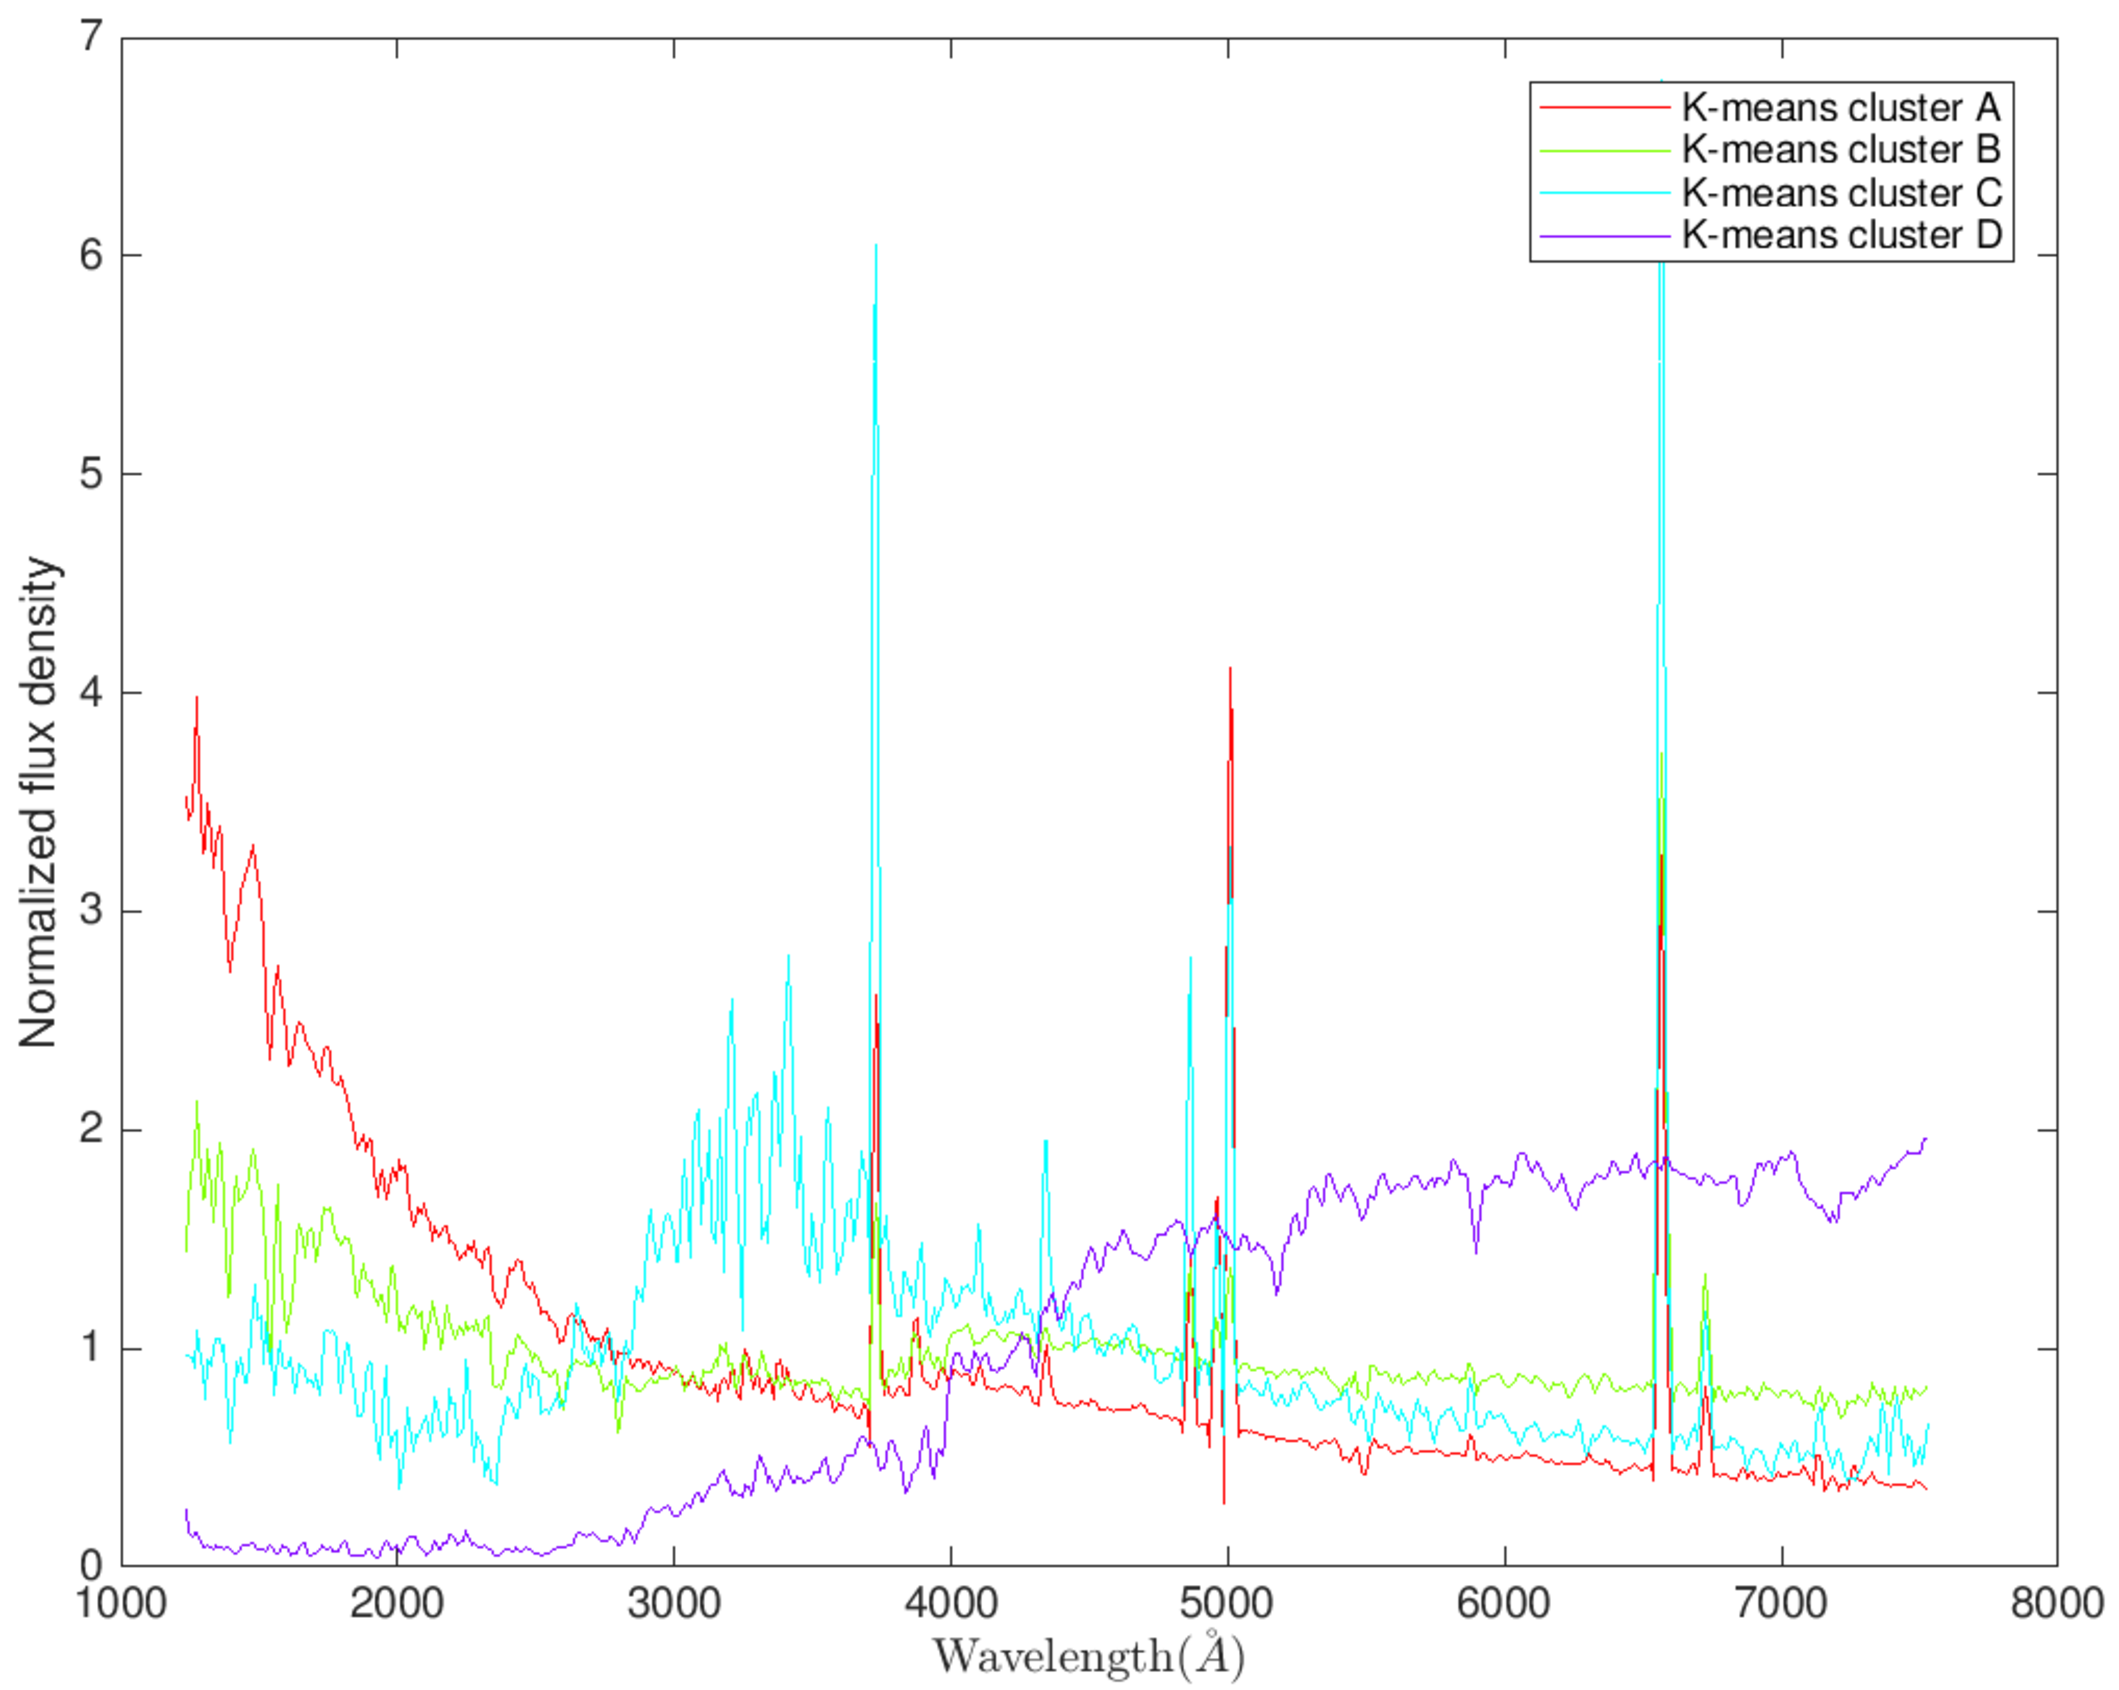
\includegraphics[width=.99\textwidth, height=         7.5cm]{k_means_images/classified_group_in_4cluster_kinney_1.pdf}
    \end{subfigure}
    \hfill
        \begin{subfigure}[b]{0.49\textwidth}
        \centering \includegraphics[width=.99\textwidth, height=         7.5cm]{k_means_images/classified_group_in_4cluster_som.png}
    \end{subfigure}
    \caption{Clustering the \citetalias{Kinney96} template spectra using K-means clustering (left) and SOM (right). Note that both methods randomly assign the initial values for their analysis, therefore the cluster labels are only used for distinguishing cluster membership.}
    \label{fig: som_k_means_4}
    \end{figure*}
        
    We performed K-means clustering on the \citetalias{Kinney96} template spectra using 4 clusters.
    Fig.~\ref{fig: som_k_means_4} shows the clustering of the template spectra into 4 groups using both K-means and SOMs.
    Both methods separated the most starburst-like and quiescent galaxies in a similar manner.
    However, they show discrepancies for spectral types between these extreme cases.
    Table~\ref{tab:kmeans_som4} shows the group assignments of the \citetalias{Kinney96} templates in the two methods.
    Templates B, E, S0 and Sa are grouped in the same cluster/neuron in both K-means and $1\times4$-sized SOM. 
    K-means grouped the Sb template with the above templates, but the SOM network classified it as a separate group, possibly because it is much more noisy in the ultraviolet range.
    The K-means method clustered the Sc template as a separate group, 
    likely due to its distinct features in the 3000--4000 \AA range, while the SOM network grouped it with SB5 and SB6. 
    Classifying the Sc template in the group with SB5 and SB6 obscures the peak feature in the Sc template.
    However, when the number of SOM nodes is increased (e.g. in Fig.~\ref{fig: 1by22T}), the Sc template separates and occupies a single neuron.
    Another noticeable difference is that K-means clustered the SB1 and SB2 templates in one group and SB3 to SB6 in another, while the SOM network grouped the SB1 to SB4 templates in one neuron and SB5 and SB6 in another.
    SB1 and S2 have similar strong emission lines in the blue, while SB3--6 show H$\alpha$ emission but only weaker emission lines at shorter wavelengths;
    the SB5 and SB6 templates are flatter with a less-pronounced 4000 \AA break than the remaining SB templates.
    By comparing the membership of different clusters in Table~\ref{tab:kmeans_som4} we can see that K-means clustering emphasizes the input templates' similarities, while SOM emphasizes the templates' differences.
     
    
    \begin{table}
    \centering
    \begin{tabular}{||l|c|c||}
    \hline
    \hline
    \citetalias{Kinney96} template & K-means group & SOM group \\
    \hline
    B                                & C               & 1                         \\
    E                                & C               & 1                         \\
    S0                               & C               & 1                         \\
    Sa                               & C               & 1                         \\
    Sb                               & C               & 2                         \\
    Sc                               & D               & 3                         \\
    SB1                              & B               & 4                         \\
    SB2                              & B               & 4                         \\
    SB3                              & A               & 4                         \\
    SB4                              & A               & 4                         \\
    SB5                              & A               & 3                         \\
    SB6                              & A               & 3                        \\
    \hline
    \end{tabular}
    \caption{Group assignments for \citetalias{Kinney96} template galaxies, using K-means and $1\times4$-sized SOM methods}
    \label{tab:kmeans_som4}
    \end{table}
 
        \subsubsection{Classifying the galaxy sample}
         \label{sec: 1Dv}
         
         After training with the templates, we used both K-means and self-organizing maps to classify the 142 galaxies in the \citetalias{Hossein12} sample.
         K-means classification was performed by assigned each galaxy to the K-means cluster with the closest centroid and the results are discussed in Section~\ref{sec: Kmeansvssomvsann}.
        This section examines the results of one-dimensional SOM-based classification in detail.
         
         
            
            The upper panel in Fig.~\ref{fig: 1by2V} shows the result of this classification using the $1\times2$~network from Fig.~\ref{fig: 1by2T}.
            Eighty of the galaxies have spectral types similar to those of the quiescent galaxies and the spectral types of the rest are similar to the starburst galaxies.
            The lower left panel shows the median spectrum of the 80 galaxies that were classified as quiescent. 
            These galaxies are similar to the ones in the left node in the upper panel of Fig.~\ref{fig: 1by2T}:
            the spectra clearly show the 4000\AA~break, one of the signatures of quiescent galaxies.
            The H$\alpha$ emission in the spectrum could be from galaxies with similar spectral types to Sa galaxies, but with stronger emission lines.
            The median spectrum in the lower right panel of Fig.~\ref{fig: 1by2V} shows strong emission lines and bright ultraviolet continuum, indications of a high star formation rate.
            \begin{figure}
                \begin{subfigure}[b]{0.45\textwidth}
                    \centering
                    \includegraphics[width=\textwidth]{images0.01/1d/hit_v_1_by_2.png}
                \end{subfigure}
                \hfill
                \begin{subfigure}[b]{0.45\textwidth}
                     \includegraphics[width=\textwidth]{images0.01/1d/SED_total1by2_fluxdensity.png}
                \end{subfigure}
                \caption{Classification of fitted galaxy spectra from \citet{Hossein12} using the $1\times2$~network trained from the \citet{Kinney96} templates (Fig.~\ref{fig: 1by2T}). Upper panel: a hit map with the number in each node representing the number of galaxies belonging to that group. In this case 80 means that 80 of the 142 spectra are classified into the quiescent group while the 62 of the 142 spectra are categorized as starburst galaxies. Lower panel: median spectra of the galaxies in each group (flux densities are normalized by dividing spectra by flux density at 4000\AA), quiescent on the left and starburst on the right.}
                \label{fig: 1by2V}
            \end{figure}          
            
            Since in this network galaxies were forced to be divided into a maximum of two groups, the strongest feature in a galaxy's spectrum predominantly decided to which group the galaxy belonged.
            Galaxies with a weak 4000~\AA~break, strong emission lines and ultraviolet upturn are categorized as starbursts while galaxies with a strong 4000~\AA~break are categorized as quiescent.
            Increasing the size of the SOM helps solve the problem of galaxies which have features that are common in both groups.
            
            Fig.~\ref{fig: 1by3V} presents the result of classifying the spectra of the galaxies using the $1\times3$~network (from Fig.~\ref{fig: 1by2T}): 66 of the galaxies belong to the quiescent group, and 47 belong to the starburst group. 
            However, 29 of the galaxies are similar to starbursts in some, but not all, of their features. 
            Galaxies in this group have strong emission lines and are ultraviolet-bright, but they also have a strong 4000~\AA~break, which makes them cluster closer to the quiescent galaxies (middle panel in the lower part of Fig.~\ref{fig: 1by2V}).

            \begin{figure}
                \begin{subfigure}[b]{0.5\textwidth}
                    \centering
                    \includegraphics[width=\textwidth]{images0.01/1d/hit_v_1_by_3.png}
                \end{subfigure}
                \hfill
                \begin{subfigure}[b]{0.5\textwidth}
                     \includegraphics[width=\textwidth]{images0.01/1d/SED_total1by3_fluxdensity.png}
                \end{subfigure}
                \caption[Classification of fitted galaxy SEDs from \citet{Hossein12} using the $1\times3$~networks]{Same as Fig.~\ref{fig: 1by2V}, but in this figure, we used a network with size of $1\times3$ (Fig.~\ref{fig: 1by3T}) to classify the sample galaxies.}
                \label{fig: 1by3V}
            \end{figure}       
            
            In Fig.~\ref{fig: 1by22V}, we use the $1\times22$~network to classify the sample galaxies.
            As mentioned in Section~\ref{sec: 1Dt}, in this network size we observed the first separation of the \citetalias{Kinney96} templates into 12 different neurons.
            As in Figs.~\ref{fig: 1by2V} and ~\ref{fig: 1by3V}, the upper panel of Fig.~\ref{fig: 1by22V} shows the number of galaxies (out of the 142) belonging to each neuron in the $1\times22$ SOM.
            The lower panels present the median spectra of the galaxies in each neuron.
            Since galaxies had more space to separate, some of the neurons are left empty.
            Thus, instead of having 22 median spectra in the lower part of Fig.~\ref{fig: 1by22V}, there are only 14.

            \begin{figure*}
                \begin{subfigure}[b]{\textwidth}
                    \includegraphics[width=\textwidth]{images0.01/1d/hit_v_1_by_22_n.png}
                    \centering
                \end{subfigure}
                \hfill
                \begin{subfigure}[b]{\textwidth}
                \centering
                     \includegraphics[width=\textwidth]{images0.01/1d/SED_total1by22_fluxdensity.png}
                \end{subfigure}
                \caption[Classification of fitted galaxy SEDs from \citet{Hossein12} using the $1\times22$~networks]{Same as Fig.~\ref{fig: 1by2V}, but in this figure, we used a network with size of $1\times22$ (Fig.~\ref{fig: 1by22T}) to classify the sample galaxies. In the median spectra of each neuron, we can clearly see the changes from quiescent galaxies to the starburst ones. The 4000\AA~ break weakens from left to right and the emission line strengths increase.}
                \label{fig: 1by22V}
            \end{figure*}
            
            Comparing the upper panel of Fig.~\ref{fig: 1by22V} with the lower panel of Fig.~\ref{fig: 1by22T} shows that the occupied neurons are not necessarily the same.
            If a cluster from the \citetalias{Hossein12} sample fills the same neuron as a \citetalias{Kinney96} template, we can conclude that the spectra of galaxies in the cluster are very similar to those of the template.
            Otherwise, we can conclude that the spectra of galaxies in the cluster are (dis)similar to two of the \citetalias{Kinney96} templates.
            For the latter case, the colours establish which template has greater similarity to the \citetalias{Hossein12} cluster.
            
            The first two neurons in the upper plot in Fig.~\ref{fig: 1by22V} are empty, while these neurons were occupied by galaxies B and E in the trained network.
            We therefore conclude that there are no galaxies in the \citetalias{Hossein12} sample with spectral type similar to that of type B or E.
            There are 3 galaxies in the third neuron, similar to the S0 type. 
            19 of the galaxies are in the fifth neuron and similar to the Sa type, while the 6 galaxies in the fourth neuron have spectral type similar to both S0 and Sa galaxies.
            There are 8 Sb type galaxies and 19 galaxies with spectral types similar to both Sa and Sb.
            The following two neurons (eighth and ninth neurons from the left) are on the edge of the quiescent and starburst galaxies.
            In the upper panel in Fig.~\ref{fig: 1by22T}, the colour between these two neurons is black, which shows that these two are very different.
            Therefore, 24 galaxies in the eighth neuron have similar spectra to Sb type galaxies, and the spectra of the 5 galaxies in the ninth neuron are similar to the SB6 galaxies.
            The far right neurons in the network belong to galaxies with spectra comparable to types SB1 and SB2.
            
            
    
   

      
    \subsection{Two-dimensional self-organizing maps}
    \label{sec: 2D}
        The one-dimensional networks are great tools to categorize the spectral types of galaxies and monitor the changes of properties of galaxies with category.
        However, each neuron in these networks is limited to connecting to one other neuron in each direction.
        In a 2D network, each neuron can have more than two immediate neighbours, providing a more complete picture of relations between spectral types.
        One of the other key features of SOMs compared to supervised classification is the ability to both interpolate between and extrapolate outside of training set classes.
        This permits a fuller exploration of dataset properties and detection of outliers.
        
        As described in Section~\ref{sec: method_somz}, one of the main advantages of the SOM is that when the weight of one neuron is adjusted after finding the best matching unit, the weight of the whole map will be changed.
        This quality of the SOMs provides a unique opportunity to analyse 2D networks using two approaches. 
        At first, as in the 1D SOMs, we assumed that all the galaxies must have spectra similar to any of the 12 templates in Fig.~\ref{fig: k96}~(i.e. no outliers).
        In this case, we can categorize spectra of other galaxies based on those 12 types.
        In the second approach, we trained networks with the assumption that there might be completely different types of galaxies not encountered before.
        This approach can be used to trace and recognize the outliers, which could include galaxy types that are not present in the \citetalias{Kinney96} templates (e.g. dwarf galaxies, luminous infrared galaxies, or active galactic nuclei).
        To execute the second approach, we used the \textsc{selforgmap} library in \textsc{matlab}.
        Unlike the \textsc{newsom} library in which the ordering step neighbourhood distance is set by default (although in an SOM it should be a free parameter), in \textsc{selforgmap} we can change this value.
        Using the \textsc{selforgmap} code, based on the size of a map and the ordering step neighbourhood distance, we can arrange that the data spread all over the SOM or sit close together, allowing room for outliers.

        To get the best result from both methods, we should have SOMs with ``enough"  neurons to give any new types of galaxies a chance to find their places in the map.
        ``Enough neurons" is a vague statement, but as mentioned in Section~\ref{sec: method_somz} the size of SOMs is arbitrary and depends on the size of the input data and the kind of information needed from the SOMs.
        Since the training dataset (the \citetalias{Kinney96} templates) has 12 members, we assumed a SOM with size of $8\times8$~would be a good start.
        We then increased the size of the SOM to find the highest size suitable for the training sample.
        We noticed that very few changes occurred after the SOMs were grown to a size greater than $12\times12$, so we used this as the maximum size.
    
        \begin{figure*}
            \begin{subfigure}[b]{0.45\textwidth}
                \centering
                \includegraphics[width=\textwidth]{images0.01/2d/dist_12_by_12.png}
            \end{subfigure}
            \hfill
            \begin{subfigure}[b]{0.45\textwidth}
                \centering
                \includegraphics[width=\textwidth]{images0.01/2d/dist_12_by_self_org_res12.png}
            \end{subfigure}
            \hfill
            \begin{subfigure}[b]{0.45\textwidth}
                \includegraphics[width=\textwidth]{images0.01/2d/hit_v_12_by_12.png}
            \end{subfigure}
            \hfill
            \begin{subfigure}[b]{0.45\textwidth}
                \includegraphics[width=\textwidth]{images0.01/2d/hit_v_12_by_self_org_res12.png}
            \end{subfigure}
            \caption[$12\times12$ two-dimensional self-organizing map results]{$12\times12$~2D SOM results. Upper panel: SOMs trained using the \citet{Kinney96} templates. For training 2D SOMs two different approaches were considered: either only 12 types of galaxies exist (left) or not (right). Lower panel: classifying the galaxies from \citet{Hossein12}, using the trained networks shown in the upper panels. From the lower right panel, we can see that there are no outliers in the galaxies from \citetalias{Hossein12}, and we can use the map in the lower left panel as a final clustering result for the \citetalias{Hossein12} galaxies.}
            \label{fig: 12by12}
        \end{figure*}
    
        The upper left panel in Fig.~\ref{fig: 12by12} shows the SOM results from the first approach. 
        Since we considered that spectra of all galaxies can be categorized using the \citetalias{Kinney96} templates, the galaxies were placed all over the map.
        Using this network to categorize any set of spectra forced the spectra to be either in the same neurons as the \citetalias{Kinney96} templates or in the neurons between them.
        In the map shown in the upper right panel in Fig.~\ref{fig: 12by12}, the \citetalias{Kinney96} templates are in a small region. This provides enough freedom for the spectra of galaxies to be placed everywhere in the map, even far away from the templates.
    
    
        In the upper left part of the map in Fig.~\ref{fig: 12by12}, although galaxies have more ways to be separated, they were separated into two main groups.
        There is a distinguishable strip of grey, dark grey and in some cases black colour in the map:
        this strip separates quiescent galaxies from starburst ones.
        The lower map shows that 5 of the neurons on the left side of the strip are full. 
        These five neurons are the same as the ones on the left hand side of Fig.~\ref{fig: 1by2T} (quiescent galaxies),
        the only difference being that in this map they have more space to be separated from each other.
        When we use this network to categorize the spectra of galaxies, any galaxy placed on the left hand side of the strip is a quiescent galaxy and any one placed on the right side of the strip is a starburst one.
        The decision about what sub-type of quiescent or starburst galaxy is based upon its position relative to each type in the SOM.
        \citetalias{Hossein12} showed that by masking emission lines (i.e., by ignoring details in spectra) two types of galaxies, Sb and SB6, can be misclassified as one another.
        As mentioned before, few-node, one-dimensional SOMs are a good method to obtain a big picture of the problem under study with less emphasis on fine detail. 
        For example, the SB6 category is placed near Sb galaxies in the 1D network in Fig.~\ref{fig: 1by22T}.
        However, in the upper left panel of Fig.~\ref{fig: 12by12}, we can see that the Sb and SB galaxies are completely separated. 
        This shows that more details of spectral shapes are considered by 2D networks, which is one of the main advantages of  using 2D maps over 1D ones.
       In this case, the two dimensions of the self-organizing map correspond approximately to quiescent versus star-forming (left to right) and less to more extinction (bottom to top). 
    
        As in the other map, in the upper right panel of Fig.~\ref{fig: 12by12}, galaxies are generally divided into two main groups.
        The border between the quiescent galaxies and the starburst ones is the black strips in the middle of the map, ending with the bright grey colour at the bottom of the map in the fifth neuron.
        In this network, neurons in the right side of the strip represent the quiescent galaxies and the neurons in the left side represent the starburst ones. 
        When categorizing a new set of spectral types, if the new spectra are similar to the \citetalias{Kinney96} templates all of them will be placed in the bottom of the map, but if the new spectra represent different types of galaxies, they would sit in any other neurons in the map.
        In large datasets, one can easily use this network to figure out whether there is any of new type of spectra (or any outliers) in the datasets. 
        Since the networks are already available, this procedure should be quick (from a few seconds to a few minutes) and easy for big datasets.
          
    
        We used both 2D networks to categorize the \citetalias{Hossein12} galaxies and the results are shown in the lower panels of Fig.~\ref{fig: 12by12}.
        In the lower right map in Fig.~\ref{fig: 12by12}, all galaxies are placed in the bottom part of the map and we can conclude that in the \citetalias{Hossein12} sample there are no outliers or spectra with very different from the \citetalias{Kinney96} templates.
        The lower left map of Fig.~\ref{fig: 12by12} shows the \citetalias{Hossein12} galaxies categorized based on the network in the upper left of Fig.~\ref{fig: 12by12}. 
        Comparing this categorization with the 1D one from Fig.~\ref{fig: 1by22V}, we can see that only 23 galaxies correspond exactly to \citetalias{Kinney96} types.
        Using 2D maps results in categorizing galaxies into more intermediate types than in 1D maps.
        In both lower maps in Fig.~\ref{fig: 12by12}, most galaxies are in the quiescent side of the SOM, which was predictable from the results in Section~\ref{sec: 1Dv}.
        This does not necessarily imply that in general there are more quiescent galaxies at higher redshift but could be a selection effect for galaxies that had more reliable redshift estimates.
        
    Although for ease of presentation this paper first discusses 1D networks and continues to 2D networks, we suggest that users of SOMs for galaxy spectral classification should use 2D networks first.
         These can be used as a first step with networks similar to the upper left map in Fig.~\ref{fig: 12by12} to identify outliers in the sample.
        After finding and removing outliers in the input data, the use of 1D and 2D maps is complementary.
        One-dimensional maps are helpful for exploring the general and ordered behaviour of the data, while 2D maps can show a more detailed picture.
 
\subsection{Comparing classification methods}
    \label{sec: Kmeansvssomvsann}
   
    The one and two-dimensional self-organizing map classifications are compared briefly above. 
    The 2-D maps allow galaxies to be members of more intermediate classes, and this is a general advantage of SOMs compared to the artificial neural network method used by \citetalias{Hossein12}: in the SOM method galaxies do not need to exactly match template spectra. 
    \citetalias{Hossein12} found that the ANN method could only match 105 out of the 142 galaxies directly to the \citetalias{Kinney96} templates; classifying the remaining 37 galaxies required combining template spectra.
    Below we compare various other classification methods with the results of the 1-D self-organizing maps using the metrics described in Section~\ref{sec:metrics}.
    Because the 2-D SOMs subdivide the sample into a larger number of groups, each containing a small number of objects, they are not directly comparable to the other methods and are not included here.
       
       To compare results from SOM, K-means, and supervised ANN, we first consider how well these methods matched a simple chi-squared fitting classification. 
        Matching galaxy spectra to templates using chi-squared, we found that not all of the templates had matches among the galaxy sample: no galaxy spectra were best-matched to the B, E, or Sc templates. 
        This is consistent with the results from the self-organized maps.
        Summing the classification score over all galaxies in the sample allows us to compare how well each technique matched the results of chi-squared fitting.
        The totals were K-means 124, $1\times4$-sized SOM 103, $1\times12$-sized SOM 111.5, $1\times22$-sized SOM 79, and supervised ANN 52.
        This shows that the K-means method and $1\times12$-sized SOM have the most similarity with minimum chi-square fitting.
        Summing the classification score over all methods for a single galaxy shows how well the methods agree for a particular spectrum.
        For example, if the total score of a galaxy is 5, it means that all techniques classified the galaxy into the same group.
        Comparing the scores, we found that 12 per cent of galaxies scored 5, 36 per cent of galaxies had a score greater than 4, and 56 per cent had a total score of 3 or more.
        The score-5 galaxies classified similarly by all methods were primarily (60 per cent) in the Sa template group. 
        The score $\geq 3$ galaxies were predominantly SB1, Sa, and Sb type (32, 28, 18 per cent, respectively).
        The different methods show the most agreement for galaxies similar to the SB1 and Sa templates, with less agreement on the high-extinction starburst types (SB5, SB6).
           
        
       We also used the Fleiss kappa index \citep{Fleiss71} to 
        measure the agreement between methods. 
        Here the `raters' are the different methods classifying a specific number of objects (i.e. 142 galaxies) to a number of classes (i.e. 12 templates).
        We computed values of Fleiss kappa twice: firstly to compare results from K-means, supervised ANN, and $1\times12$-sized SOM and secondly to compare results from K-means, supervised ANN, and $1\times22$-sized SOM.
        The resulting values were $\sim 27$ per cent and $\sim 21$ per cent, respectively.
        According to \citet{landis77}, the interpretation of a Fleiss kappa measure in the range 21--40 per cent is that the raters are in fair agreement, consistent with the results above. 

A final comparison between the classification methods is 
made with the silhouette score  \citep{rousseeuw87}.
The highest score among our classification was for K-means (0.549), followed by $1\times4$-sized SOM (0.371), $1\times12$-sized SOM (0.302) and $1\times22$-sized SOM (0.249).
The chi-squared fitting resulted in a score of 0.221 and the supervised neural network 0.142.
As discussed in Section~\ref{sec:metrics}, the silhouette score usually declines as the number of groups increases, so we cannot conclude from these values that K-means is the superior method. 
However, the $1\times12$-sized SOM, chi-squared fitting, and supervised neural network all have either 8 or 9 classes.
In this case we can compare scores directly and conclude that the self-organized map yields groups with more internal similarity.
This is in contrast to the comparison between K-means and self-organized maps for the templates alone (see Section~\ref{sec: Kmeansvssom}) where K-means clustering  produced groups more similar to each other, and emphasizes that the exact data used in a clustering process can strongly affect the outcome.


 \subsection{Properties of spectral groups}
       
       \begin{figure*}
            \centering
            \includegraphics[width=\textwidth]{images0.01/1d/props5.png}
            \caption[The median of four properties of galaxies in three networks]{Comparing the median of four properties of galaxies in each node in $1\times2$ (black circles), $1\times4$ (blue diamonds), and $1\times8$ (red triangles) networks.}
            \label{fig: props}
        \end{figure*} 
        
       To check whether the classifications described above are meaningful, in this section we examine the relations between median properties of the galaxies in each group. 
          Fig.~\ref{fig: props} shows the median of stellar mass, age, specific star formation rate (sSFR; star formation rate per stellar mass), and $f_\mathrm{burst}$ of the galaxies in each neuron in the $1\times2$, $1\times4$, and $1\times8$ self-organized map networks.
        In all plots, the horizontal axis is the number of the neurons divided by the size of the network.
        As shown in Fig.~\ref{fig: props}, in all three networks, stellar mass and age decrease while sSFR and $f_\mathrm{burst}$ increase as the type changes from quiescent galaxies to starburst.
       Separating galaxies based on spectral types also leads to a separation in properties derived (via {\em CIGALE}) from the SEDs, as expected since the spectral types are also based on {\em CIGALE} fitting. 
    

        {\em CIGALE} has various models to derive the properties of galaxies.
        Through these models, some of the properties are already known to be correlated with each other, e.g., stellar mass and star formation rate.
        \citetalias{Noll09} studied other relations between properties with no direct correlation in the models in a sample of SINGS galaxies.
        They found a tight correlation between sSFR and t$_{\rm {D4000}}$, which suggests that younger stellar population correlates with higher SFR.
        They also found correlations between stellar mass and SFR, and stellar mass and t$_{\rm {D4000}}$.
        Since in the {\em CIGALE} code, stellar mass is a free parameter, \citetalias{Noll09} argued that any stellar-mass-related correlation must be astrophysically meaningful. 
        They also studied relations between the attenuation at 1500 \AA~(A$_{\rm {FUV}}$) and sSFR, age, and stellar mass and did not find any correlation.
        \citetalias{Hossein12} replicated the upper plots in Fig.~\ref{fig: props_vs_props}, and found a tighter correlation than in the \citetalias{Noll09} results. 
        
        \begin{figure*}
\includegraphics[width=\textwidth]{images0.01/1d/fig11_new_col.png}
        \caption{
        From top to bottom: relations between age (t$_{\rm {D4000}}$) and sSFR ($\phi$), sSFR and stellar mass, age (t$_{\rm {D4000}}$) and stellar mass, and A$_{\rm {FUV}}$ with sSFR, age (t$_{\rm {D4000}}$) and stellar mass. 
        Circles, pentagons, and squares show the median values of these properties of galaxies in the $1\times22$, $1\times 12$ and $1\times4$ SOM networks; 
        triangles show the median value of properties for each K-means cluster (using $K=4$) and stars show median values for groups from \citetalias{Hossein12}.
        Error bars show standard deviations of the group properties.
        Colours show the galaxy types in the SOM classification. 
        The lightest grey (most pure red in the online version) colour shows E type galaxies and the black (most blue in the online version) indicates the SB1 galaxies. 
        The shading of other colours between light grey and black (red and blue in the online version) measures the location of galaxies along the SOM from  quiescent to starburst.}
        \label{fig: props_vs_props}
        \end{figure*}
    
        To compare our classifications with previous work, Fig.~\ref{fig: props_vs_props} shows plots similar to those shown by both \citetalias{Noll09} and \citetalias{Hossein12}.
        The points represent the median values of the properties of the galaxies in each group, with different symbol types representing classification method and error bars indicating the standard deviation of those properties.
       The colour scale represents neuron number in the SOM method, shading from quiescent to starburst. 
        The medium grey (purple in the online version) point in the middle of the black (blue in the online version) points in Fig.~\ref{fig: props_vs_props} corresponds to galaxies with spectra similar to type Sc: the shape of their spectra indicates that they are old galaxies with high sSFR.
        
        Overall, Fig.~\ref{fig: props} and the upper panels in Fig.~\ref{fig: props_vs_props} show the same trends as noted by \citetalias{Noll09} and \citetalias{Hossein12}:
        galaxies with lower mass tend to be younger and more active.
        The median group properties as derived by all of the methods show high Pearson correlation coefficients ($r^2\gtrsim 0.9$) between the quantities shown.
        The ordering of groups in the SOM maps also corresponds to an ordering in age:    
        from older to younger galaxies, the colour of the points changes from light grey to black (red to blue in the online version).
        
        \citetalias{Noll09} studied relations between A$_{\rm {FUV}}$ and other properties of galaxies and found that the attenuation had no dependence on the specific star formation or age.
        In contrast to \citetalias{Noll09}, we find a correlation between A$_{\rm {FUV}}$ and these two parameters, shown in the lower panels of Fig.~\ref{fig: props_vs_props}.
        Although weaker then the correlations above, Pearson correlation coefficients are higher for the SOM groups than for other methods, particularly for the $1x12$-sized SOM. 
        The slightly different distribution of this particular classification (see Fig.~\ref{fig: 1by12T}) classifies the most quiescent objects as similar to slightly more active galaxies, lessening the turnover in properties as A$_{\rm {FUV}}$ increases.
        
        The general sense of the correlation between A$_{\rm {FUV}}$ and sSFR in Fig.~\ref{fig: props_vs_props} is similar to the trend found by \cite{Dale07}.
        They used IR luminosity to UV luminosity ratio (L$_{IR}$/L$_{FUV}$) as a measure of A$_{\rm {FUV}}$ and compared it with sSFR for all 75 galaxies in the SINGS survey.
        They found that for quiescent galaxies (E, S0 and S0/a), L$_{IR}$/L$_{FUV}$ (or A$_{\rm {FUV}}$) correlates with sSFR, and for spiral galaxies, there is an anticorrelation between L$_{IR}$/L$_{FUV}$ and sSFR.
        Since our sample has no E-type galaxies, we cannot confidently claim the same relation between A$_{\rm {FUV}}$ and sSFR. 
        However, Fig.~\ref{fig: props_vs_props} does indicate an increase in A$_{\rm {FUV}}$ with increasing sSFR for the quiescient types and a decrease with increasing sSFR for the starburst types.
        Both \cite{Dale07} and \citetalias{Noll09} argued that these apparent trends can be a result of the dependence of star formation history on L$_{IR}$/L$_{FUV}$.
        Whether this dependence is real or not, our results here show that using self-organizing maps can separate spectra of galaxies in such a way that the characteristics of each of these groups are in agreement with the general picture of galaxy evolution.
          
       One of the key features of SOMs is the ability to not only classify objects but to provide an {\em ordered} classification.
       K-means clustering and supervised ANNs can sort galaxy spectra into classes but do not naturally order them. Ordering is important in the case where the physical causes of the differences between classes/clusters are unknown. Average properties of objects within clusters (possibly from data not used for classification) can be used to test hypotheses about the physical differences. 
       Figures~\ref{fig: props} and~\ref{fig: props_vs_props} show that the SOM ordering also corresponds to the ordering of the physical properties of the galaxy models used to make the classified spectra. 
       The median properties of the spectral groups change on going from one end of the SOM to the other.
       Therefore, by using the SOM method, we can study not only how galaxies group into spectral clusters, but the trends between the clusters as well.